\section{Experimental Results}

In the following, we explore the effects of tuning WHERE, Random Forest,
and CART. LR will be used, untuned, in order to check one of the recommendations
made by Hall et al.~\cite{hall11}.

\subsection{RQ1:  Does  Tuning  Improve Performance? }\label{sect:precision}


\fig{deltas} says  that the answer to RQ1 is ``yes''-- tuning  has a positive effect on performance scores. This figure sorts
 deltas in the precision and the F-measure    between tuned and untuned learners. Our reading of this
figure is that, overall, tuning rarely makes performance   worse and often can make it much better. 
 

\begin{figure}[!t]
\begin{center}
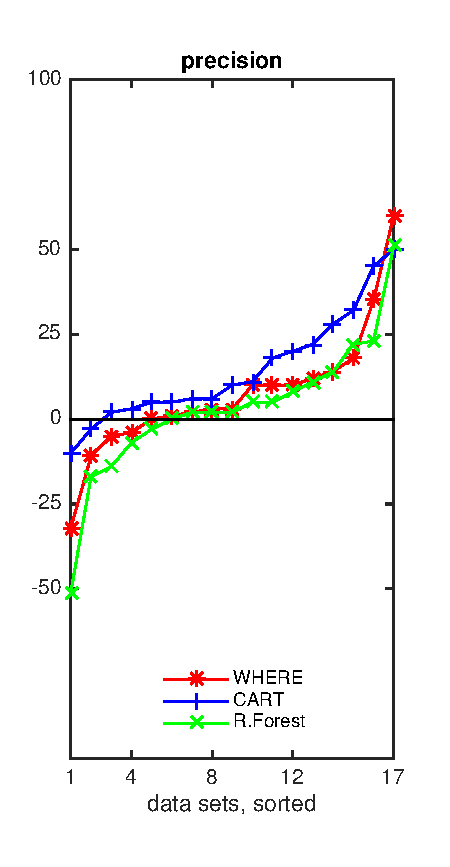
\includegraphics[width=1.5in]{./eps/improvements_precision.eps}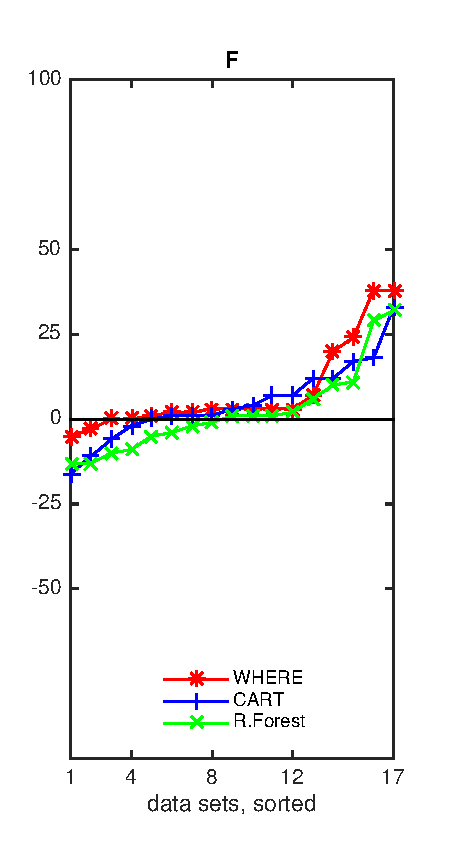
\includegraphics[width=1.5in]{./eps/improvements_F.eps}
 \end{center}
\caption{Deltas in performance  seen in \tab{precisionbars} (left)
and \tab{fbars} (right) between tuned and untuned learners. Tuning improves performance when the deltas are above zero.}\label{fig:deltas}
 \end{figure}
 
 
\tab{precisionbars} and \tab{fbars} show the
the specific values seen before and after tuning with {\em precision}
and {\em ``F''} as different optimization goals(the corresponding  ``F'' and precision values for
\tab{precisionbars} and \tab{fbars} are not provided for the space limitation).
For each data set, the maximum precision or ``F'' values for each data set are shown in {\bf bold}.
As might have been
 predicted by Lessmann et al.~\cite{lessmann2008benchmarking}, 
untuned CART is indeed the worst learner (only one of its
untuned results is best and {\bf bold}). 
And, 
in $\frac{12}{17}$ cases, the  untuned Random Forest performs better than or equal to untuned CART in terms of precision.  
% Note that the size of the improvement is sometimes small; e.g. the precision results improve more than the ``F'' measure.
% But even when the {\em median} change is small, there still may exist
% interesting (i.e.  exceptionally
% large) improvements from tuning-- for example, 
%  see the last  two ``F'' improvements for WHERE in \fig{deltas} where the improvements were greater than 70\%.
% Some of the data sets in \fig{precisionbars} proved challenging for all learners;
% e.g. the precision results for {\em ivy} are less
% that impressive.
% To some extent, this is due to
% the properties of   the data set (as shown in \fig{data1}, defective classes in {\em ivy} are very rare in tuning data).




That said,  tuning can improve those poor performing detectors.
In some cases, the median changes may be small (e.g. the ``F'' results for WHERE and Random Forests) but even in
those cases, there are enough large changes to motivate the use of tuning. For example:
\bi
\item
For ``F'' improvement, there are two improvements over 25\% for both WHERE and Random Forests. Also, in {\em poiV0}, all untuned learners report ``F'' of under 50\%, tuning changes those scores by 25\%. Finally, note the  {\em xercesV1} result for the WHERE learner. Here, tuning changes precision from 32\% to 70\%.
\item
Regarding precision, for {\em antV0}, and {\em antV1} untuned WHERE reports precision of 0. But tuned WHERE scores 35 and 60 (the similar pattern can seen in ``F'').

\ei

% To complete the discussion in this section, we note that in the Lessmann et al. study,  Random Forest dramatically out-performed CART.
% In this study, we show that  
% tuned CART is now comparable to Random Forest. So our new results
% do not complete reverse the results of Lessmann et al. However, they
% do show that the Lessmann results are ``brittle'', in the sense that
% tuning can remove the effect they report.

\begin{table}[!t]
\renewcommand{\baselinestretch}{0.8} 
% \centering
\scriptsize    

\begin{tabular}{r|rl|rl|rl|rl|rl|rlrl}
%\begin{tabular}{r@{~}|r@{~}l@{~}|r@{~}l@{~}|r@{~}l|r@{~}l@{~}|r@{~}l@{~}|r@{~}l@{~}r@{~}l}
      &   \multicolumn{4}{c|}{WHERE}         &   \multicolumn{4}{c|}{CART}         &   \multicolumn{4}{c}{Random Forest}         \\\hline
  Data set   &   \multicolumn{2}{c}{default}         &   \multicolumn{2}{c|}{Tuned}         &   \multicolumn{2}{c}{default}         &   \multicolumn{2}{c|}{Tuned}    &   \multicolumn{2}{c}{default}  &   \multicolumn{2}{c}{Tuned}\\\hline
antV0 & 0 &   & 35 &   & 15 &   & {\bf 60} &   & 21 &   & 44 &  \\
antV1 & 0 &   & 60 &   & 54 &   & 56 &   & {\bf 67} &   & 50 &  \\
antV2 & 45 &   & 55 &   & 42 &   & 52 &   & 56 &   & {\bf 67} &  \\
camelV0 & 20 &   & 30 &   & 30 &   & 50 &   & 28 &   & {\bf 79} &  \\
camelV1 & 27 &   & 28 &   & {\bf 38} &   & 28 &   & 34 &   & 27 &  \\
ivy & 25 &   & 21 &   & 21 &   & {\bf 26} &   & 23 &   & 20 &  \\
jeditV0 & 34 &   & 37 &   & 56 &   & {\bf 78} &   & 52 &   & 60 &  \\
jeditV1 & 30 &   & 42 &   & 32 &   & {\bf 64} &   & 32 &   & 37 &  \\
jeditV2 & 4 &   & {\bf 22} &   & 6 &   & 17 &   & 4 &   & 6 &  \\
log4j & 96 &   & 91 &   & 95 &   & 98 &   & 95 &   & {\bf 100} &  \\
lucene & 61 &   & 75 &   & 67 &   & 70 &   & 63 &   & {\bf 77} &  \\
poiV0 & 70 &   & 70 &   & 65 &   & {\bf 71} &   &  67 &   & 69 &  \\
poiV1 & 74 &   & 76 &   & 72 &   & 90 &   & 78 &   & {\bf 100} &  \\
synapse & 61 &   & 50 &   & 50 &   & {\bf 100} &   & 60 &   & 60 &  \\
velocity & 34 &   & {\bf 44} &   & 39 &   & {\bf 44} &   & 40 &   & 42 &  \\
xercesV0 & 14 &   & 17 &   & 17 &   & 14 &   & {\bf 28} &   & 14 &  \\
xercesV1 & 86 &   & 54 &   & 72 &   & {\bf 100} &   & 78 &   & 27 &  \\
\end{tabular}
\caption{Precision results (best results  shown in {\bf bold}).}
\label{tab:precisionbars}
\end{table}
 

\begin{table}[!t]
\renewcommand{\baselinestretch}{0.8} 
% \centering
\scriptsize  
~~~\begin{tabular}{r|rl|rl|rl|rl|rl|rlrl}
      &   \multicolumn{4}{c|}{WHERE}         &   \multicolumn{4}{c|}{CART}         &   \multicolumn{4}{c}{Random Forest}         \\\hline
  Data set   &   \multicolumn{2}{c}{default}         &   \multicolumn{2}{c|}{Tuned}         &   \multicolumn{2}{c}{default}         &   \multicolumn{2}{c|}{Tuned}    &   \multicolumn{2}{c}{default}  &   \multicolumn{2}{c}{Tuned}\\\hline
antV0 & 0 &   & 20 &   & 20 &   & {\bf 40} &   & 28 &   & 38 &  \\
antV1 & 0 &   & 38 &   & 37 &   & {\bf 49} &   & 38 &   & {\bf 49} &  \\
antV2 & 47 &   & 50 &   & 45 &   &  49 &   & {\bf 57} &   & 56 &  \\
camelV0 & 31 &   & 28 &   & 39 &   & 28 &   & {\bf 40} &   & 30 &  \\
camelV1 & 34 &   & 34 &   & 38 &   & 32 &   & {\bf 42} &   & 33 &  \\
ivy & 39 &   & 34 &   & 28 &   & {\bf 40} &   & 35 &   &  33 &  \\
jeditV0 & 45 &   & 47 &   & 56 &   & 57 &   & {\bf 63} &   & 59 &  \\
jeditV1 & 43 &   & 44 &   & 44 &   & 47 &   & 46 &   & {\bf 48} &  \\
jeditV2 & 8 &   & {\bf 11} &   & 10 &   & 10 &   & 8 &   & 9 &  \\
log4j & 47 &   & 50 &   & 53 &   & 37 &   & {\bf 60} &   & 47 &  \\
lucene & 73 &   & 73 &   & 65 &   & 72 &   & 70 &   & {\bf 76} &  \\
poiV0 & 50 &   & 74 &   & 31 &   & 64 &   & 45 &   & {\bf 77} &  \\
poiV1 & 75 &   & {\bf 78} &   & 68 &   & 69 &   & 77 &   & {\bf 78} &  \\
synapse & 49 &   & 56 &   & 43 &   & {\bf 60} &   & 52 &   & 53 &  \\
velocity & 51 &   & 53 &   & 53 &   & 51 &   & {\bf 56} &   & 51 &  \\
xercesV0 & 19 &   & 22 &   & 19 &   & {\bf 26} &   & 34 &   & 21 &  \\
xercesV1 & 32 &   & 70 &   & 34 &   & 35 &   & 42 &   & {\bf 71} &  \\
\end{tabular}
\caption{F-measure results (best results  shown in {\bf bold}).}
\label{tab:fbars}
\end{table}

\subsection{RQ2:  Does Tuning Change a Learner's Ranking ?}\label{sect:rank}
Researchers often use performance criteria to assert that one learner is better than 
another~\cite{lessmann2008benchmarking,me07b,hall11}. For example:
\be
\item
Lessmann et al.~\cite{lessmann2008benchmarking} conclude that
Random Forest is considered to be statistically 
better than CART. 
\item
Also, in Hall et al.'s   systematic literature review\cite{hall11}, it is argued
that defect predictors based on simple 
modeling techniques such as LR perform better than complicated techniques such as Random Forest\footnote{By three measures,
Random Forest
is more complicated than LR. Firstly, LR builds one model
while Random Forest builds many models. Secondly, LR is just
a model construction tool while Random Forest needs both
a tool to construct its forest {\em and} a second tool
to  infer some conclusion from all the members of that forest.
Thirdly, the LR model can be printed in a few lines while the multiple
models learned by Random
Forest model would take up multiple pages of output.}.
\ee
Given tuning, how stable are these  conclusions?
Before answering issue, we digress for two comments.



Firstly, it is important to comment on why it is  so important to check the conclusions
of these particular papers. 
These  papers are prominent publications (to say the least).
Hall et al.~\cite{hall11} is the fourth most-cited IEEE TSE
paper for 2009 to 2014 with 176 citations (see goo.gl/MGrGr7)
while the Lessmann et al. paper~\cite{lessmann2008benchmarking} has 394 citations (see
goo.gl/khTp97)-- which is quite remarkable for a paper published in 2009.
Given the prominence
of these papers, researchers might believe it is
appropriate to
  use  their advice without testing that advice on local data sets.

Secondly, while we are critical of the results of
Lessmann et al. and Hall et al., it needs to be said that  their analysis  was 
excellent and exemplary given the state-of-the-art of the tools used when those papers were written.  
While Hall et al. did not perform any new experiments, 
their
summarization of so many defect prediction papers have not been equalled
before (or since).
As to the Lessmann et al. paper, they  compared
22 data miners using various   data sets (mostly from NASA)~\cite{lessmann2008benchmarking}.
In that study, some learners were tuned using manual methods 
(C4.5, CART and Random Forest)
and some, like SVM-Type learners, were tuned by automatic grid search (for more on grid search, see   {\S}2.1).



\begin{figure}[!t]
% \begin{center}
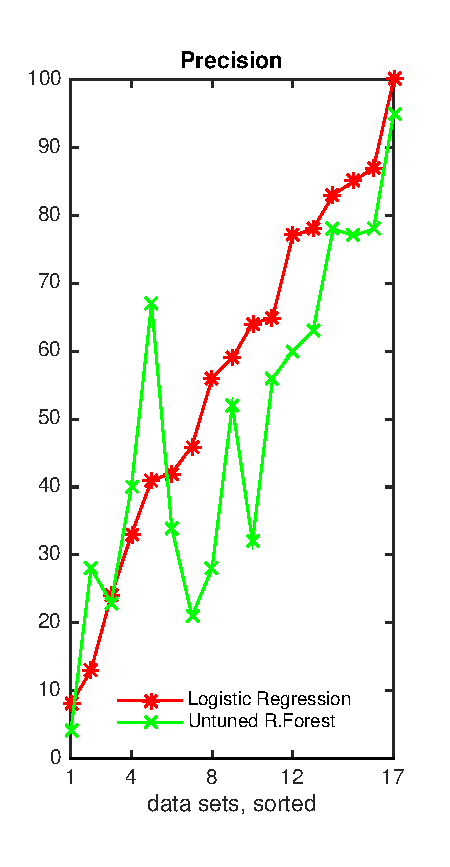
\includegraphics[width=1.5in]{./eps/LR_untuned.eps}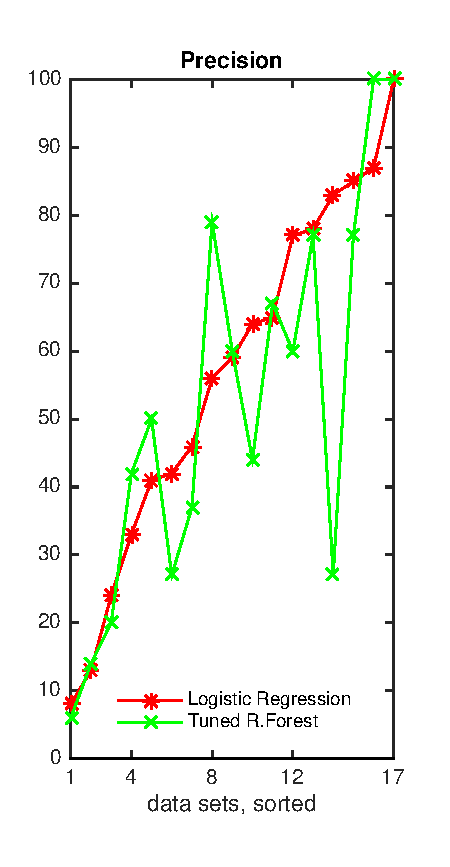
\includegraphics[width=1.5in]{./eps/LR_tuned.eps}
%  \end{center}
\caption{Comparison between Logistic Regression and Random Forest before and after tuning. }\label{fig:lr}
 \end{figure}
 
 
That said, our tuning results show that it is time to revise
the recommendations of those papers. 
  \fig{lr} comments on the advice from Hall et al. (that LR is better than Random Forest)L
  \bi
  \item
 In a result that might have been predicted by Hall et al.,  
 untuned Random
Forests performs comparatively worse than
 Logistic Regression. Specifically, untuned
 Random Forest performs worse than Linear regression in in 13 out of   17 data sets. 
\item
However, it turns out that advice is sensitive to the tunings
used with Random Forest. After tuning, we find that tuned Random Forest
loses to Logistic Regression in only 6 out of 17 data sets. 
\ei

As to Lessmann et al.'s advice (that Random Forest is better than 
CART),  
in \tab{precisionbars} and \tab{fbars}, we saw those counter-examples
to that statement.
Recall in those tables,
tuned CART are better than or equal
to tuned Random Forest in $\frac{12}{17}$ and $\frac{7}{17}$ data sets in
terms of precision and F-measure, respectively. Prior to tuning experiments, those
numbers are $\frac{5}{17}$ and $\frac{1}{17}$. Results from the non-parametric
Kolmogorov-Smirnov(KS) Test show that the performance 
scores of tuned CART and tuned Random Forest are not statistically different.
Note that Random Forest is  not significantly better than CART, would not have been
predicted by   Lessmann et al.
  

Hence we answer RQ2 as ``yes'': tuning can change how  data miners are comparatively ranked.
 


% \begin{figure}[!t]
% \begin{center}
% 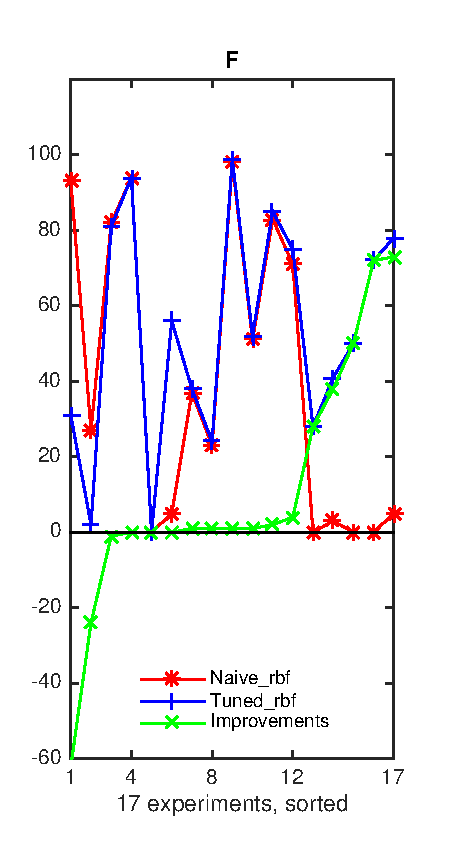
\includegraphics[width=1.5in]{svm_rbf.eps}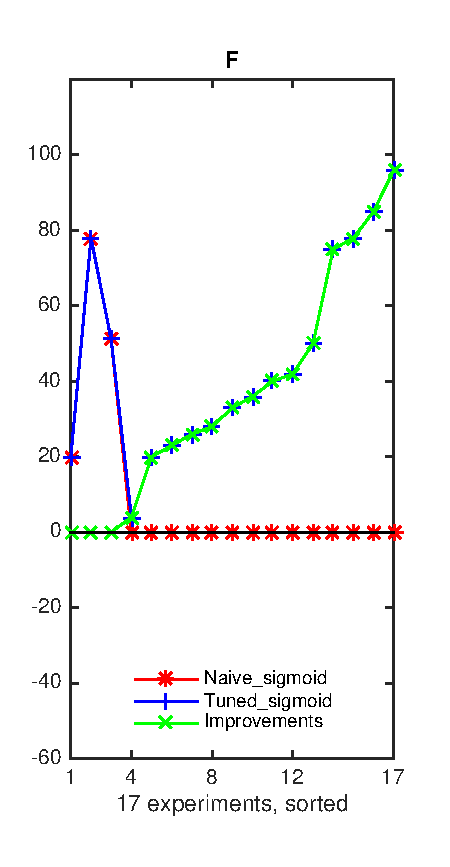
\includegraphics[width=1.5in]{svm_sigmoid.eps}
%  \end{center}
% \caption{Comparison between tuned and naive SVM learners with rbf and sigmoid kernels over the goal of F. }\label{fig:svm}
%  \end{figure}








 \subsection{RQ3: Does Tuning Select Different Project Factors? }\label{sect:import}


Researchers often use data miners to  test what factors have most impact on software projects~\cite{bell2013limited,rahman2013how,me02k,Moser:2008,zimmermann2007predicting,herzig2013predicting}. 
\tab{features} comments that such tests are unreliable since the factors selected by a data miner are much altered before and 
after tuning.

\tab{features} shows what features are found in the trees generated by the WHERE algorithm
(bold shows the features found by the trees from tuned WHERE; plain text shows the features seen
in the untuned study). Note that different features are selected depending on whether or not
we tune an algorithm.


% list some features
\begin{table}[!t]

\renewcommand{\baselinestretch}{0.8}
\scriptsize
\centering
  \begin{tabular}{c|p{1in}|p{1in}}
    \multicolumn{1}{c|}{ Data set}  &   \multicolumn{1}{c|}{Precision} & \multicolumn{1}{c}{F} \\ \hline 
 \multirow{2}{*}{antV0} & {\bf rfc} &  {\bf None} \\
         & mfa, loc, cam, dit, dam, lcom3 & mfa, loc, cam, dit, dam, lcom3\\
  \hline
 \multirow{2}{*}{camelV0} & {\bf mfa, wmc, lcom3} &{\bf None }\\
        & mfa, wmc, rfc, loc, cam, lcom3 & mfa, wmc, rfc, loc, cam, lcom3\\
  \hline
 \multirow{2}{*}{ivy} & {\bf cam, dam, npm, loc, rfc, wmc} &{\bf cam, dam, npm, loc, rfc, wmc }  \\
       & loc, cam, dam, wmc, lcom3 & loc, cam, dam, wmc, lcom3 \\
  \hline
 \multirow{2}{*}{jeditV0} &{\bf mfa, dam, loc }&{\bf mfa, dam, loc}\\
         & mfa, lcom3, dam, dit, ic & mfa, lcom3, dam, dit, ic \\
  \hline
 \multirow{2}{*}{log4j} & {\bf loc, ic, dit }&{\bf mfa, wmc, rfc, loc, npm}\\
         & mfa, lcom3, loc, ic & mfa, lcom3, loc, ic \\
   \hline
  \multirow{2}{*}{lucene} & {\bf dit, cam, wmc, lcom3, dam, rfc, cbm, mfa, ic} & {\bf dit, lcom3, dam, mfa}\\
         & dit, cam, dam, ic & dit, cam, dam, cbm, ic\\
   \hline
   \multirow{2}{*}{poiV0} & {\bf mfa, amc, dam }& {\bf mfa, amc, dam} \\
        & mfa, loc, amc, dam, wmc, lcom & mfa, loc, amc, dam, wmc, lcom\\
   \hline
   \multirow{2}{*}{synapse} &{\bf loc, dit, rfc, cam, wmc, dam, lcom,  mfa,  lcom3} & {\bf dam} \\
        & loc, mfa, cam, lcom, dam, lcom3 & loc, mfa, cam, lcom, dam, lcom3\\
    \hline
   \multirow{2}{*}{velocity} & {\bf dit, wmc, cam, rfc, cbo, moa, dam }& {\bf mfa, dit }\\
        & dit, dam, lcom3, ic, mfa, cbm  & dit, dam, lcom3, ic, mfa\\
    \hline
   \multirow{2}{*}{xercesV0} &{\bf  wmc }&{\bf cam, dam, avg\_cc, loc, wmc,  dit,  mfa, ce, lcom3 }\\
        & wmc, mfa, lcom3, cam, dam &  wmc, mfa, lcom3, cam, dam \\
    \hline
    
  \end{tabular}
  
    \caption{Features selected by tuned WHERE with different goals:
    {\bf bold} features are those found useful by the tuned WHERE.
    Also, features shown in plain text are those found useful by the untuned WHERE.
    }\label{tab:features}
\end{table}


For example, consider {\em mfa} which is the
number of methods inherited by a class plus the number of methods accessible by member methods of the class.
For both goals (precision and ``F'') {\em mfa} is selected for 8 and 5 data sets,
for the untuned and tuned data miner (respectively).
Similar differences are   seen with other attributes.


As to why different tunings select for different features,  recall from {\S}2.1 that tuning changes how data miners
heuristically explore a large space of possible models. As we change how that exploration proceeds,
so we change what features are found by that exploration.

In any case, our answer to RQ3 is ``yes'', tuning changes our
conclusions about what factors are most important in software engineering.
Hence, many old papers    need to be revisited  and perhaps revised~\cite{bell2013limited,rahman2013how,me02k,Moser:2008,zimmermann2007predicting,herzig2013predicting}.  
For example, one of us (Menzies) used data miners
to assert that some factors were more important than others for predicting
successful software reuse~\cite{me02k}. That assertion should now be doubted since Menzies did not conduct a tuning study before reporting what factors the data miners
found were most influential.

\begin{figure}[!t]
% \begin{center}
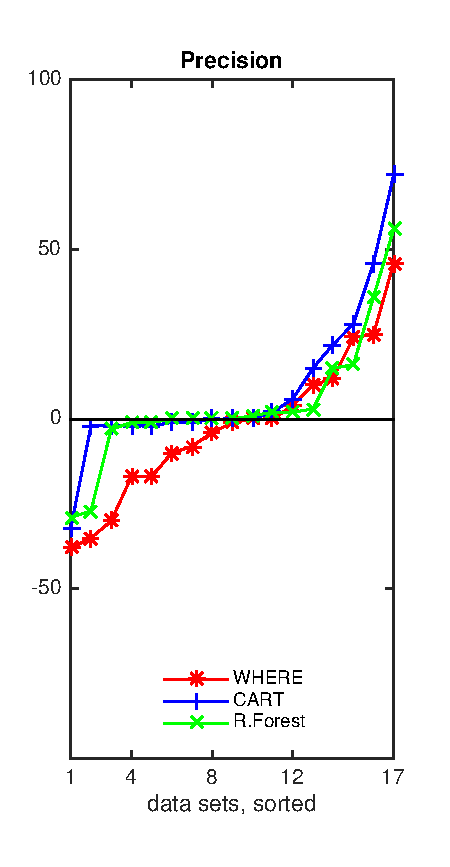
\includegraphics[width=1.5in]{./eps/np_precision.eps}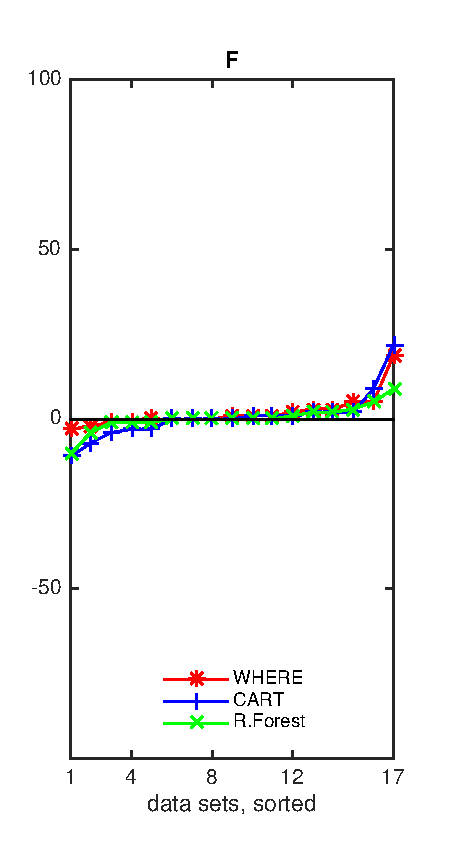
\includegraphics[width=1.5in]{./eps/np_f.eps}
%  \end{center}
\caption{Deltas in performance between {\em np = 10} and the recommended np's. The recommended np is better when deltas are above zero. {\em np = 90, 50 and 60} are recommended population size for WHERE, CART and Random Forest by Storn.}\label{fig:deltas_np}
 \end{figure}



\subsection{RQ4: Is Tuning Easy?}\label{sect:easy}

In terms of the search space
explored via tuning, optimizing defect prediction from static code
measures is much {\em smaller} than the standard optimization.

To see this,
recall from Algorithm~1 that
DE explores a {\em Population} of size {\em np = 10}. This is a very small population size since
Rainer Storn (one of the inventors of DE) recommends  setting {\em np} to be ten times larger than the number
of attributes being optimized~\cite{storn1997differential}.

From \tab{parameters},
we see that Storn would therefore recommend {\em np} values of
90, 50, 60 for WHERE, CART and Random Forest (respectively). Yet we achieve our results
using a constant {\em np = 10}; i.e. $\frac{10}{90}, \frac{10}{50}, \frac{10}{60}$ of the
recommended search space.

To justify that {\em np = 10} is enough, we did another tuning study, 
where all the settings were the same as before but we set {\em np = 90, np = 50} and {\em np = 60} for WHERE, CART and Random Forest, respectively (i.e. the settings
as recommended by Storn). The tuning performance of learners was evaluated
by precision and ``F'' as before. To compare performance of each learner with different {\em np}'s, we computed the delta in the performance between {\em np = 10} and {\em np} using any of \{90, 50, 60\}.

Those deltas, shown in \fig{deltas_np}, are sorted along the x-axis. In those plots, a zero or negative $y$ value means that {\em np = 10} performs as well or better than  {\em np $\in \{90, 50, 60\}$}. One technical aside: the data set orderings in \fig{deltas_np} on the x-axis are not the same (that is,
if {\em np $>$ 10} was useful for optimizing one data set's precision score, it was not necessary for that data set's F-measure score).

  \fig{deltas_np} shows that
the median improvement is zero; i.e. {\em np = 10} usually does as well as anything else. This observation is
supported by the   KS
  results of \tab{ks}. At a 95\% confidence, the
KS threshold  is $1.36\sqrt{34/(17*17)} = 0.46$, which is greater than  the values in \fig{deltas_np}. That is, no result in  \fig{deltas_np} is significantly different to any other-- which is to say that
there is no evidence that   {\em np = 10} is a poor choice of search space size.

Another measure showing that tuning is easy 
(for static code defect predictors)
is the number of evaluations required to complete optimization
(see next section). That is, we answer RQ4 as ``yes'', tuning is surprisingly easy-- at least
for defect predictors and using DE.


% \begin{table}[!t]
% \centering
% \scriptsize
% \begin{tabular}{|l|c|c|}
% \hline
% Learner & CART & WHERE \\ \hline
% CART    & -    & 0.42  \\ \hline
% R.Forest      & 0.29 & 0.18  \\ \hline
% \end{tabular}
% \begin{tabular}{|l|c|c|}
% \hline
% Learner & CART & WHERE \\ \hline
% CART    & -    & 0.24  \\ \hline
% R.Forest      & 0.24 & 0.29  \\ \hline
% \end{tabular}
% \caption{Kolmogorov-Smirnov Tests for numbers seen in \fig{deltas_np}: Precision(left) and F(right).}
% \end{table}


\begin{table}[!t]
\renewcommand{\baselinestretch}{0.8}
\scriptsize
 \centering
  \begin{tabular}{c|c c|cc}
    &   \multicolumn{2}{c|}{Precision} & \multicolumn{2}{c}{F} \\ \hline 
    Learner & CART  & WHERE & CART & WHERE \\
\hline
    CART & - & 0.41 & - & 0.24 \\
    R. Forest &  0.12 & 0.35 & 0.18 & 0.18 \\
  \end{tabular}
    \caption{Kolmogorov-Smirnov Tests for distributions of  \fig{deltas_np}}\label{tab:ks}
\end{table}

\begin{figure}[!t]
\begin{center}
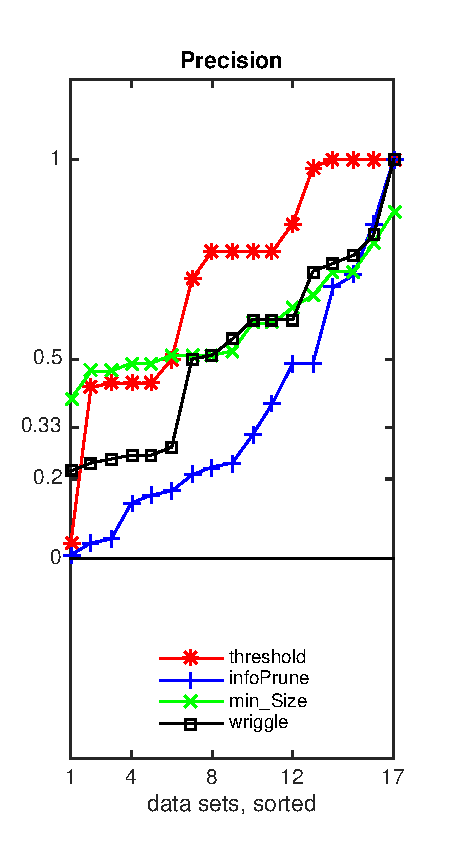
\includegraphics[width=1.5in]{./eps/features_precision.eps}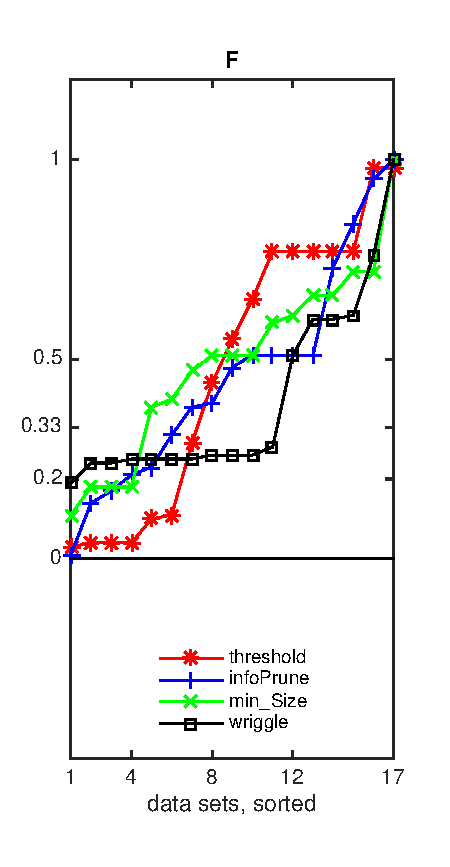
\includegraphics[width=1.5in]{./eps/features_F.eps}
\end{center}
\caption{Four representative tuning values in WHERE with  precision and F-measure as the tuning goal, respectively.   }\label{fig:features}
 \end{figure}

% \begin{table}[!t]
% \renewcommand{\baselinestretch}{0.8}
% \scriptsize
% \centering
%   \begin{tabular}{c|c |c}
%     &   \multicolumn{1}{c|}{Precision} & \multicolumn{1}{c}{F} \\ \hline 
%     Learner  & np = 10 & recommended np \\
% \hline
%     WHERE & 0.18 & 0.24 \\
%     CART  & 0.12 & 0.12  \\
%     R. Forest &  0.12 & 0.12 \\
%   \end{tabular}
%     \caption{Kolmogorov-Smirnov Tests for distributions of each learner with np = 10 and recommended np's }\label{tab:ks}
% \end{table}

% %%% repalce this table with the new one
% \begin{table}[!ht]

% \renewcommand{\baselinestretch}{0.8}
% \scriptsize
% \centering
%   \begin{tabular}{c|c c|c c|c c|c c| c c }
  
%     &   \multicolumn{2}{c|}{Precision} & \multicolumn{2}{c|}{F} &  \multicolumn{2}{c|}{SUM}\\
%  &&&&&&&\\
% Features&   
%   default
% & tuned
% & default
% & tuned
% & default
% & tuned
% \\\hline

% max\_cc& & & &  & & \\
% noc& & & & & & \\
% ca& & & & & & \\
% cbo& & 1& & & & 1\\
% moa& & 1& & & & 1\\
% ce& & 2& & 1& & 3\\
% avg\_cc& & 2& & 2& & 4\\
% npm& 1& 2& 1& 1&2 & 3\\
% lcom& 1& 2& 1& 1& 2& 3\\
% amc& 4& 2& 4& 2& 8& 4\\
% cbm& 5& 2& 5& 3& 10& 5\\
% rfc& 3& 6& 3& 8& 6& 14\\
% wmc& 5& 4& 5& 9& 10& 13\\
% dit& 8& 3& 7& 7& 15& 10\\
% ic& 8& 3& 8& 6& 16 & 9\\
% lcom3& 8& 6& 8& 8&16 & 14\\
% cam& 9& 7& 9& 7& 18& 14\\
% loc& 9& 5& 9& 11& 18& 16\\
% dam& 13& 6& 13& 11& 26& 17 \\
% mfa& 16& 9& 16& 9&32 & 18\\

 
%   \end{tabular}
%     \caption{Counts of features selected by different goals.Given that we are processing 17 data sets, the maximum counts for any 
% one cell in the ``precision'' or ``F'' column is 17.  
%     }\label{tab:counts}
% \end{table}
 

% \begin{table*}[!ht]

% \renewcommand{\baselinestretch}{0.75}
% \scriptsize
% \centering
%   \begin{tabular}{r|c |c |c |c |c |c }
%     Datasets & Tuned\_Where & Default\_Where & Tuned\_CART & Default\_CART & Tuned\_RanFst & Default\_RanFst\\
%     \hline
%     antV0 & 50 / 90.18 & 1.57 & 60 / 4.36 & 0.09 & 50 / 8.12 & 0.18\\
%     antV1 & 50 / 174.67 & 2.90 & 50 / 6.35 & 0.10 & 50 / 11.77 & 0.27\\
%     antV2 & 50 / 403.63 & 6.92 & 70 / 9.71 & 0.16 & 60 / 13.28 & 0.35\\
%     camelV0 & 50 / 537.53 & 8.60 & 50 / 9.14 & 0.18 & 50 / 13.73 & 0.31\\
%     camelV1 & 60 / 1640.54 & 24.57 & 60 / 17.06 & 0.24 & 70 / 31.53 & 0.73\\
%     ivy & 70 / 77.75 & 1.02 & 60 / 3.86 & 0.06 & 50 / 8.00 & 0.17\\
%     jeditV0 & 80 / 472.57 & 5.49 & 60 / 6.30 & 0.09 & 70 / 13.01 & 0.30\\
%     jeditV1 & 60 / 489.45 & 6.82 & 70 / 7.61 & 0.11 & 60 / 12.87 & 0.32\\
%     jeditV2 & 50 / 435.43 & 7.21 & 50 / 6.46 & 0.12 & 90 / 20.34 & 0.37\\
%     log4j & 70 / 113.73 & 1.36 & 70 / 3.25 & 0.05 & 60 / 7.07 & 0.16\\
%     lucene & 70 / 224.39 & 2.70 & 50 / 4.07 & 0.08 & 50 / 8.87 & 0.26\\
%     poiV0 & 60 / 261.06 & 4.00 & 60 / 6.23 & 0.10 & 50 / 10.57 & 0.29\\
%     poiV1 & 80 / 607.85 & 7.18 & 60 / 7.69 & 0.13 & 50 / 11.39 & 0.29\\
%     synapse & 50 / 116.04 & 1.87 & 60 / 4.07 & 0.05 & 70 / 9.74 & 0.16\\
%     velocity & 60 / 195.27 & 2.75 & 60 / 4.49 & 0.06 & 80 / 12.15 & 0.21\\
%     xercesV0 & 60 / 143.69 & 2.17 & 70 / 7.26 & 0.09 & 60 / 10.28 & 0.23\\
%     xercesV1 & 50 / 794.50 & 13.37 & 50 / 8.24 & 0.15 & 60 / 14.54 & 0.38\\

%   \end{tabular}
%   \caption{Evaluations/runtimes and runtimes for tuned and default learners(in sec), optimizing for  precision.  }\label{tab:etimes}
% \end{table*}
% %%%%time for F %%%%%%
% \begin{table*}[!ht]
% \renewcommand{\baselinestretch}{0.75}
% \scriptsize
% \centering
%   \begin{tabular}{r|c |c |c |c |c |c } 
%     Datasets & Tuned\_Where & Default\_Where & Tuned\_CART & Default\_CART & Tuned\_RanFst & Default\_RanFst\\
%     \hline
%     antV0 & 50 / 94.08 & 1.71 & 60 / 4.55 & 0.08 & 60 / 10.79 & 0.21\\
%     antV1 & 60 / 193.74 & 3.02 & 70 / 7.77 & 0.09 & 60 / 12.30 & 0.25\\
%     antV2 & 80 / 643.94 & 7.59 & 60 / 8.38 & 0.15 & 70 / 16.99 & 0.41\\
%     camelV0 & 60 / 662.56 & 9.97 & 60 / 13.19 & 0.23 & 80 / 26.11 & 0.32\\
%     camelV1 & 60 / 1800.64 & 24.25 & 50 / 15.02 & 0.28 & 50 / 28.52 & 0.78\\
%     ivy & 60 / 69.95 & 1.03 & 50 / 3.35 & 0.08 & 70 / 9.40 & 0.18\\
%     jeditV0 & 90 / 553.80 & 5.58 & 50 / 5.58 & 0.09 & 60 / 15.08 & 0.33\\
%     jeditV1 & 60 / 519.75 & 8.76 & 50 / 7.43 & 0.13 & 60 / 18.13 & 0.41\\
%     jeditV2 & 70 / 621.32 & 8.98 & 50 / 9.71 & 0.15 & 60 / 17.38 & 0.63\\
%     log4j & 70 / 125.29 & 1.73 & 50 / 2.90 & 0.06 & 60 / 8.76 & 0.19\\
%     lucene & 50 / 221.99 & 3.52 & 50 / 5.20 & 0.10 & 50 / 10.09 & 0.33\\
%     poiV0 & 60 / 327.48 & 5.13 & 50 / 6.56 & 0.11 & 50 / 12.88 & 0.36\\
%     poiV1 & 50 / 523.85 & 8.95 & 80 / 12.26 & 0.14 & 60 / 19.56 & 0.35\\
%     synapse & 70 / 148.23 & 1.91 & 60 / 3.96 & 0.06 & 60 / 8.19 & 0.16\\
%     velocity & 50 / 156.51 & 2.75 & 60 / 4.27 & 0.06 & 50 / 7.70 & 0.22\\
%     xercesV0 & 60 / 142.83 & 2.01 & 70 / 7.15 & 0.08 & 60 / 9.61 & 0.20\\
%     xercesV1 & 50 / 751.92 & 12.98 & 60 / 9.28 & 0.16 & 50 / 12.69 & 0.38\\

%   \end{tabular}
%   \caption{Evaluations/runtimes and runtimes for tuned and default learners(in sec), optimizing for F-measure.  }\label{tab:ftimes}
% \end{table*}




%%%%time for prec %%%%%%
\begin{table*}[!ht]
\renewcommand{\baselinestretch}{0.75}
\scriptsize
\centering
  \begin{tabular}{r|c |c |c |c |c |c }
    Datasets & Tuned\_Where & Naive\_Where & Tuned\_CART & Naive\_CART & Tuned\_RanFst & Naive\_RanFst\\
    \hline
    antV0 & 50 / 95.47 & 1.65 & 60 / 5.08 & 0.08 & 60 / 9.78 & 0.20\\
    antV1 & 60 / 224.67 & 3.03 & 50 / 6.52 & 0.12 & 60 / 14.13 & 0.25\\
    antV2 & 70 / 644.99 & 8.24 & 50 / 9.00 & 0.24 & 60 / 16.75 & 0.44\\
    camelV0 & 70 / 690.62 & 7.93 & 70 / 12.68 & 0.24 & 110 / 28.49 & 0.34\\
    camelV1 & 60 / 1596.77 & 23.56 & 60 / 17.13 & 0.27 & 70 / 33.96 & 0.77\\
    ivy & 60 / 66.69 & 0.97 & 60 / 4.26 & 0.07 & 60 / 8.89 & 0.19\\
    jeditV0 & 80 / 459.30 & 5.33 & 80 / 8.69 & 0.11 & 90 / 18.40 & 0.32\\
    jeditV1 & 60 / 421.56 & 6.59 & 80 / 9.05 & 0.12 & 80 / 17.93 & 0.36\\
    jeditV2 & 90 / 595.56 & 6.88 & 60 / 7.90 & 0.14 & 110 / 27.34 & 0.38\\
    log4j & 50 / 76.09 & 1.33 & 50 / 2.60 & 0.06 & 80 / 9.69 & 0.15\\
    lucene & 80 / 236.45 & 2.60 & 70 / 6.07 & 0.10 & 60 / 9.77 & 0.25\\
    poiV0 & 60 / 263.12 & 3.92 & 70 / 7.42 & 0.09 & 130 / 25.86 & 0.28\\
    poiV1 & 50 / 398.33 & 6.94 & 70 / 9.31 & 0.13 & 50 / 12.67 & 0.29\\
    synapse & 70 / 144.09 & 1.85 & 50 / 3.88 & 0.07 & 50 / 8.13 & 0.19\\
    velocity & 60 / 184.10 & 2.68 & 50 / 4.27 & 0.07 & 100 / 15.18 & 0.21\\
    xercesV0 & 60 / 136.87 & 1.98 & 80 / 9.17 & 0.10 & 70 / 14.17 & 0.22\\
    xercesV1 & 80 / 1173.92 & 12.78 & 60 / 10.47 & 0.16 & 50 / 18.27 & 0.40\\
  \end{tabular}
  \caption{Evaluations/runtimes and runtimes for tuned and default learners(in sec), optimizing for precision.}
  \label{tab:etimes}
\end{table*}


%%%%time for F %%%%%%
\begin{table*}[!ht]
\renewcommand{\baselinestretch}{0.75}
\scriptsize
\centering
  \begin{tabular}{r|c |c |c |c |c |c }
    Datasets & Tuned\_Where & Naive\_Where & Tuned\_CART & Naive\_CART & Tuned\_RanFst & Naive\_RanFst\\
    \hline
    antV0 & 50 / 93.38 & 1.39 & 50 / 3.52 & 0.08 & 70 / 9.89 & 0.17\\
    antV1 & 60 / 186.95 & 3.18 & 50 / 6.18 & 0.12 & 60 / 13.39 & 0.25\\
    antV2 & 90 / 654.34 & 8.08 & 60 / 8.79 & 0.18 & 120 / 27.56 & 0.36\\
    camel & 50 / 543.28 & 9.65 & 80 / 17.00 & 0.28 & 70 / 22.52 & 0.41\\
    camelV1 & 60 / 1808.03 & 26.98 & 110 / 31.92 & 0.28 & 70 / 37.00 & 0.85\\
    ivy & 60 / 74.50 & 1.18 & 60 / 4.72 & 0.08 & 60 / 10.39 & 0.21\\
    jeditV0 & 80 / 518.47 & 6.11 & 60 / 7.9
 & 0.10 & 60 / 14.32 & 0.37\\
    jeditV1 & 70 / 576.29 & 6.89 & 70 / 8.13 & 0.10 & 70 / 17.42 & 0.34\\
    jeditV2 & 80 / 657.59 & 7.93 & 70 / 10.34 & 0.15 & 80 / 20.20 & 0.40\\
    log4j & 70 / 123.48 & 1.59 & 50 / 2.92 & 0.08 & 50 / 7.67 & 0.17\\
    lucene & 60 / 219.02 & 3.68 & 60 / 6.89 & 0.12 & 70 / 13.06 & 0.35\\
    poiV0 & 60 / 314.53 & 4.82 & 60 / 7.80 & 0.10 & 80 / 19.29 & 0.32\\
    poiV1 & 50 / 446.05 & 7.55 & 50 / 7.62 & 0.14 & 110 / 27.23 & 0.36\\
    synapse & 60 / 138.75 & 1.83 & 60 / 4.87 & 0.08 & 90 / 13.29 & 0.17\\
    velocity & 60 / 211.88 & 3.13 & 60 / 5.51 & 0.10 & 60 / 11.58 & 0.27\\
    xercesV0 & 80 / 178.49 & 2.02 & 60 / 7.47 & 0.11 & 80 / 17.31 & 0.28\\
    xercesV1 & 80 / 1370.89 & 14.42 & 60 / 11.07 & 0.19 & 80 / 25.27 & 0.46\\
  \end{tabular}
  \caption{Evaluations/runtimes and runtimes for tuned and default learners(in sec), optimizing for F-Measure.}
\label{tab:ftimes}
\end{table*}





\subsection{RQ5: Is Tuning Impractically Slow?}\label{sect:fast}
 
 
The number of evaluations/runtimes used by our optimizers is shown in \tab{etimes}
and \tab{ftimes}.
WHERE's runtimes are slower than CART and Random Forest since WHERE has yet to benefit from decades
of implementation experience with these older algorithms. For example, SciKitLearn's  CART and Random Forest
 make extensive use of an underlying C library whereas WHERE is a purely interpreted Python.

Looking over \tab{etimes} and \tab{ftimes}, the general pattern is that 50 to 80 evaluations suffice for finding the tuning
improvements reported in this paper. 
50 to 80 evaluations are  much fewer than our pre-experimental intuition.
Prior to this paper, the authors have conducted numerous explorations of evolutionary algorithms
for search-based SE applications~\cite{krall15,krall15:hm,fea02a,me07f,Green}. Based
on that work, our expectations were that non-parametric evolutionary optimization would
take thousands, if not millions, of evaluations of candidate tunings. This turned out not
to be that case.

Hence, we answer RQ5 as ``no'': tuning is so fast that
it could (and should) be used by anyone using defect predictors. 
%The possible reason that tuning is so fast is that the searching space for defect prediction is not complicated, which might result from the tuning range set for each parameter in \tab{parameters}.  

As to why DE can tune defect predictors so quickly, that is an
open question. One possibility is that the search space within
the control space of these data miners has  many accumulative effects such that one
decision can cascade into another (and the combination of decisions
is better than each separate  one). DE would be a natural  tool for reasoning
about such ``cascades'', due to the way it mashes candidates together,
then inserts the result back into the frontier (making them available
for even more mashing at the next step of the inference).


\subsection{RQ6: Should we use ``off-the-shelf'' Tunings?}\label{sect:variance}
 
 In \fig{features}, we show how tuning selects the optimal values for tuned parameters. For space limitation, only four parameters from WHERE learner are selected as representatives and all the others can be found in our online support documents\footnote{\url{https://goo.gl/aHQKtU}}.
 Note that
 the tunings learned were different in different data sets and for different goals.
Also, the tunings learned by DE
were often very different to the default (the default values for {\em threshold}, {\em infoPrune}, {\em min\_Size} and {\em wriggle} are $0.5$, $0.33$, $0.5$ and $0.2$, respectively). That is, to achieve the performance improvements seen in the paper,
the default tuning parameters required a wide range of adjustments.

Hence, we answer RQ6 as ``no'' since, to achieve the improvements seen in this paper, tuning has to be repeated whenever the goals or data
sets are changed. Given this requirement to repeatedly run tuning, it is fortunate that (as shown above)
tuning is so easy and so fast (at least for defect predictors from static code attributes).


 
% %%%%parameters for prec %%%%%%
% \begin{table*}[!ht]
 
% \renewcommand{\baselinestretch}{0.9}
% \resizebox{\textwidth}{!}{
% \scriptsize
% \centering
%   \begin{tabular}{|c |c |c |c |c |c |c |c |c |c |c |c |c |c |c |c |c |c |c |c |}
%     \hline
%   \begin{tabular}[c]{@{}c@{}}Learner \\ Name\end{tabular}&Parameters  & Default &antV0&antV1&antV2&camelV0&camelV1&ivy&jeditV0&jeditV1&jeditV2&log4j&lucene&poiV0&poiV1&synapse&velocity&xercesV0&xercesV1\\ 
%  \hline
% \multirow{8}{*}{\begin{tabular}[c]{@{}c@{}}Where\\based\\ Learner\end{tabular}}
% & threshold& 0.5& 0.98& 0.98& 0.43& 0.24& 0.64& 1& 1& 0.98& 0.98& 1& 1& 0.87& 0.59& 0.98& 1& 0.98& 0.98\\ \cline{2-20}
% & infoPrune& 0.33& 0.05& 0.05& 0.71& 0.54& 0.45& 0.41& 0.3& 0.05& 0.05& 0.54& 0.84& 0.01& 1& 0.05& 0.68& 0.43& 0.05\\ \cline{2-20}
% & min\_sample\_size& 4& 7& 7& 9& 8& 6& 10& 1& 5& 7& 8& 7& 9& 3& 7& 7& 1& 7\\ \cline{2-20}
% & min\_Size& 0.5& 0.51& 0.51& 0.59& 0.46& 0.13& 0.38& 0.66& 0.27& 0.51& 0.46& 0.47& 0.77& 0.48& 0.51& 0.66& 0.22& 0.51\\ \cline{2-20}
% & wriggle& 0.2& 0.6& 0.6& 0.83& 0.52& 0.19& 0.01& 0.26& 0.6& 0.6& 0.52& 0.19& 0.83& 0.01& 0.6& 0.26& 0.55& 0.6\\ \cline{2-20}
% & depthMin& 2& 1& 1& 2& 3& 5& 2& 3& 3& 1& 1& 2& 4& 2& 1& 3& 2& 1\\ \cline{2-20}
% & depthMax& 10& 8& 8& 13& 19& 19& 18& 7& 8& 8& 19& 1& 19& 18& 8& 11& 18& 8\\ \cline{2-20}
% & wherePrune& False& False& False& False& False& True& True& False& False& False& False& False& True& True& False& False& True& False\\ \cline{2-20}
% & treePrune& True& False& False& False& True& True& True& False& False& False& True& True& False& False& False& False& True& False\\ \cline{2-20}
% \hline
% \multirow{4}{*}{CART}
% & threshold& 0.5& 0.69& 0.99& 1& 0.3& 0.83& 1& 0.99& 0.58& 0.72& 1& 0.71& 0.46& 0.72& 1& 0.85& 1& 0.64\\ \cline{2-20}
% & max\_feature& None& 0.01& 0.58& 0.65& 0.66& 0.73& 0.67& 0.56& 0.01& 0.97& 0.54& 0.52& 0.32& 0.01& 0.74& 0.73& 0.01& 0.1\\ \cline{2-20}
% & min\_samples\_split& 2& 7& 16& 18& 5& 11& 6& 15& 6& 17& 4& 16& 12& 5& 14& 11& 4& 10\\ \cline{2-20}
% & min\_samples\_leaf& 1& 13& 14& 10& 4& 3& 15& 16& 9& 6& 7& 6& 1& 4& 6& 7& 11& 7\\ \cline{2-20}
% & max\_depth& None& 14& 1& 41& 34& 1& 22& 29& 1& 1& 1& 14& 19& 8& 40& 4& 1& 1\\ \cline{2-20}
% \hline
% \multirow{6}{*}{\begin{tabular}[c]{@{}c@{}}Random \\ Forests\end{tabular}} 
% & threshold& 0.5& 0.84& 0.9& 0.83& 0.33& 1& 0.99& 0.91& 1& 1& 0.83& 0.98& 0.9& 0.86& 0.83& 1& 1& 1\\ \cline{2-20}
% & max\_feature& None& 0.61& 0.13& 0.89& 0.37& 0.01& 0.98& 0.52& 0.75& 0.35& 0.01& 0.98& 0.84& 0.73& 0.01& 0.48& 0.51& 0.01\\ \cline{2-20}
% & max\_leaf\_nodes& None& 37& 35& 38& 21& 36& 45& 10& 38& 10& 30& 20& 43& 11& 13& 15& 39& 10\\ \cline{2-20}
% & min\_samples\_split& 2& 8& 16& 17& 13& 14& 2& 3& 2& 2& 18& 19& 9& 4& 4& 9& 20& 1\\ \cline{2-20}
% & min\_samples\_leaf& 1& 19& 5& 2& 4& 2& 4& 7& 17& 7& 16& 12& 2& 3& 2& 2& 2& 3\\ \cline{2-20}
% & n\_estimators& 100& 138& 112& 77& 74& 125& 130& 107& 85& 96& 111& 103& 82& 59& 149& 150& 63& 58\\ \cline{2-20}
% \hline  \end{tabular}
% }
%   \caption{Parameters tuned on different models over the objective of precision.}\label{tab:preselect}
% \end{table*}


% %%%%parameters for F %%%%%%
% \begin{table*}[!ht]
 
% \resizebox{\textwidth}{!}{
% \renewcommand{\baselinestretch}{0.9}
% \scriptsize
% \centering
%   \begin{tabular}{|c |c |c |c |c |c |c |c |c |c |c |c |c |c |c |c |c |c |c |c |}
%     \hline
    
%   \begin{tabular}[c]{@{}c@{}}Learner \\ Name\end{tabular}&Parameters  & Default &antV0&antV1&antV2&camelV0&camelV1&ivy&jeditV0&jeditV1&jeditV2&log4j&lucene&poiV0&poiV1&synapse&velocity&xercesV0&xercesV1\\ 
%  \hline
% \multirow{8}{*}{\begin{tabular}[c]{@{}c@{}}Where\\based\\ Learner\end{tabular}}
% & threshold& 0.5& 0.04& 0.44& 0.44& 0.98& 0.65& 0.77& 1& 0.65& 0.98& 0.44& 0.44& 0.87& 0.04& 0.77& 0.24& 0.44& 0.77\\ \cline{2-20}
% & infoPrune& 0.33& 0.51& 0.68& 0.88& 0.47& 0.07& 0.31& 0.48& 0.68& 0.57& 0.12& 0.68& 0.01& 0.51& 0.14& 0.54& 0.68& 0.14\\ \cline{2-20}
% & min\_sample\_size& 4& 6& 4& 6& 1& 6& 8& 8& 4& 6& 7& 4& 9& 6& 2& 8& 4& 8\\ \cline{2-20}
% & min\_Size& 0.5& 0.18& 0.4& 0.56& 0.51& 0.65& 0.59& 0.97& 0.4& 0.51& 0.8& 0.4& 0.77& 0.18& 0.62& 0.46& 0.4& 0.66\\ \cline{2-20}
% & wriggle& 0.2& 0.25& 0.29& 0.76& 0.6& 0.63& 0.26& 1& 0.51& 0.17& 0.36& 0.51& 0.83& 0.25& 0.5& 0.52& 0.29& 0.26\\ \cline{2-20}
% & depthMin& 2& 3& 3& 3& 1& 5& 3& 2& 3& 5& 5& 3& 4& 3& 3& 3& 3& 3\\ \cline{2-20}
% & depthMax& 10& 16& 15& 15& 8& 19& 10& 7& 15& 5& 15& 15& 19& 16& 6& 19& 15& 10\\ \cline{2-20}
% & wherePrune& False& False& True& True& True& True& True& True& False& False& True& True& True& False& True& False& False& True\\ \cline{2-20}
% & treePrune& True& False& True& True& False& False& False& False& False& True& True& True& False& False& False& True& True& False\\ \cline{2-20}
% \hline
% \multirow{5}{*}{CART}
% & threshold& 0.5& 0.34& 0.25& 0.01& 0.01& 0.73& 0.53& 0.92& 0.8& 0.74& 0.54& 0.03& 0.91& 0.01& 0.01& 0.55& 1& 0.01\\ \cline{2-20}
% & max\_feature& None& 0.01& 0.01& 0.29& 0.01& 0.46& 0.75& 0.79& 0.74& 0.41& 0.81& 0.61& 0.72& 0.01& 0.01& 0.01& 0.25& 0.18\\ \cline{2-20}
% & min\_samples\_split& 2& 18& 20& 12& 2& 15& 11& 2& 18& 13& 9& 17& 16& 10& 4& 8& 3& 15\\ \cline{2-20}
% & min\_samples\_leaf& 1& 19& 16& 15& 17& 1& 1& 13& 10& 4& 3& 7& 5& 20& 7& 8& 1& 6\\ \cline{2-20}
% & max\_depth& None& 12& 2& 15& 1& 41& 20& 44& 15& 13& 5& 23& 14& 1& 5& 17& 47& 13\\ \cline{2-20}
% \hline
% \multirow{6}{*}{\begin{tabular}[c]{@{}c@{}}Random \\ Forests\end{tabular}} 
% & threshold& 0.5& 0.01& 0.35& 0.3& 0.01& 0.9& 0.97& 0.63& 1& 0.73& 0.68& 0.01& 1.0& 0.01& 0.07& 0.22& 1& 0.82\\ \cline{2-20}
% & max\_feature& None& 0.63& 0.17& 0.01& 0.01& 0.88& 0.74& 0.76& 0.73& 0.01& 0.03& 0.39& 0.02& 0.01& 0.56& 0.36& 0.51& 0.89\\ \cline{2-20}
% & max\_leaf\_nodes& None& 40& 33& 46& 22& 11& 16& 38& 34& 30& 31& 12& 49& 25& 47& 15& 39& 24\\ \cline{2-20}
% & min\_samples\_split& 2& 10& 16& 20& 1& 1& 1& 1& 4& 20& 19& 11& 14& 2& 17& 19& 20& 19\\ \cline{2-20}
% & min\_samples\_leaf& 1& 4& 15& 9& 13& 18& 11& 3& 16& 17& 6& 10& 7& 19& 13& 11& 2& 14\\ \cline{2-20}
% & n\_estimators& 100& 120& 73& 75& 130& 97& 144& 125& 97& 80& 111& 96& 101& 50& 67& 74& 63& 66\\ \cline{2-20}
% \hline  \end{tabular}
% }
%   \caption{Parameters tuned on different models over the objective of ``F''.}\label{tab:fselect}
% \end{table*}



% \section{Guidelines \wei{added!}}

% As discussed above, tuning is helpful and easy to do. Any defect prediction study based on data mining should include a tuning study. However, if tuning is not done properly, performance may not be improved but degraded to some extent. Here're some tips for tuning:

% {\em Tuning Data} is important for the whole tuning process. If available data size for the study is very small, k-fold cross evaluation method can be used to split data and generate new training data as well as tuning data. On the other hand, if the study concerns more about chronology, incremental learning approach can be adopted. 


% {\em Tuning Range} will determine how large the searching space the tuner will explore and how good the parameter got from tuning. The recommended range will set the default value as the median of the range with a reasonable distance. If the performance from tuning dose not better than the default parameter, adjust ranges accordingly.

% {\em Searching algorithm} is the engine of the tuning process. Since tuning has to be repeatedly done for different goals and different data sets, simple searching algorithms, like DE and Generic algorithms, are good choice to complete this task. Other more advanced algorithms, like NSGA III \cite{deb2014evolutionary} and GALE\cite{krall15}, can also be used if multi-objective tuning is considered.